\documentclass[review]{elsarticle}

\usepackage{lineno,hyperref}
\modulolinenumbers[5]

%% May or May not 
%\usepackage{epsfig}
%\usepackage{subfigure}
%\usepackage{calc}
\usepackage{amssymb}
\usepackage{amstext}
\usepackage{amsmath}
\usepackage{amsthm}
%\usepackage{multicol}
%\usepackage{pslatex}
%\usepackage{apalike}
\usepackage{url} 
%% 

\journal{Journal of Applied Energy} % or, Journal of Energy 

%% `Elsevier LaTeX' style
\bibliographystyle{elsarticle-num}
%%%%%%%%%%%%%%%%%%%%%%%

\begin{document}

%% simple comment command 
\newcommand{\todo}[1]{\textbf{TODO: #1}\\}

\begin{frontmatter}

%\title{An Investigation Process for Hybrid Energy Grid Optimization}

\title{An Investigation Process for Hybrid Energy Grid Optimization}\tnoteref{mytitlenote}}
\tnotetext[mytitlenote]{This paper is an extended version of
  conference paper published in \cite{}. We extended our previous work
  with details on simulation models and co-simulation technology, and
  with the first actual investigation results from one case study. }  
% \author{Tae-Gil Noh, Daniel Schwabeneder,  Sebastien Nicolas, Anett
%   Sch\"ulke, } 
% \ead{tae-gil.noh@neclab.eu, schwabeneder@eeg.tuwien.ac.at,
%   sebastien.nicolas@neclab.eu, Anett.Schuelke@neclab.eu}

%% Group authors per affiliation:
% \author{Elsevier\fnref{myfootnote}}
% \address{Radarweg 29, Amsterdam}
% \fntext[myfootnote]{Since 1880.}

\author[NLE]{Tae-Gil Noh}
\ead{tae-gil.noh@neclab.eu}

\author[TUWien]{Daniel Schwabeneder}
\ead{schwabeneder@eeg.tuwien.ac.at}

\author[AIT]{Daniele Basciotti}
\ead{Daniele.Basciotti@ait.ac.at}

\author[AIT]{Sawsan Henein}
\ead{Sawsan.Henein@ait.ac.at}

\author[AIT]{Edmund Widl}
\ead{Edmund.Widl@ait.ac.at}

\author[NLE]{Sebastien Nicolas}
\ead{sebastien.nicolas@neclab.eu}

\author[TUWien]{Hans Auer}
\ead{auer@eeg.tuwien.ac.at}

\author[NLE]{Anett Sch\"ulke\fnref{corr}}
\ead{anett.schuelke@neclab.eu}

\address[NLE]{NEC Laboratories Europe, Kurfuersten-Anlage 36, 69115,
  Heidelberg, Germany}
\address[TUWien]{(address of EEG), TU Wien, Vienna, Austria}
\address[AIT]{(address of AIT), Vienna, Austria} 

\fntext[corr]{Corresponding Author}

\begin{abstract}
A hybrid energy network is an energy system operated across different
domains of energy grids, where energy can be transformed between the
grids. Hybrid energy networks can provide a way of managing volatile 
renewable energy sources. The paper introduces an investigation
process that is designed to develop and evaluate co-operative hybrid
energy network. The proposed investigation process consists of
two-step holistic investigation with simulation-based and
economic-model based analysis. The process is designed to enable
multi-aspect investigation on the range of flexibility provided by
evolution of hybrid energy grids. The paper first outlines details of
the process, including adopted simulations, co-simulation technology,
control optimization methods and economy models. Then, it reports
investigation results from one case study. 
\end{abstract}

\begin{keyword}
Hybrid Energy Network, Co-simulation, Economic Modeling, 
Cooperative Control Strategy
%\texttt{elsarticle.cls}\sep \LaTeX\sep Elsevier \sep template
%\MSC[2010] 00-01\sep  99-00
\end{keyword}
\end{frontmatter}

\linenumbers

\section{Introduction}
% \begin{verbatim}
% + Goal: why we do what we do. 
% + Problems and our answers
%   show the several blocks that prohibit us to just go and
%   investigate hybrid grid.
%   + obviously hard on real world and also hard on 
%     simulation ==> ans: co-simulation 
%   + problem of "synthetic world" ==> ans: 
%     modeling real-cities as-is first, and start from there. 
%   + hybrid-grid is more than technical ==> 
%     ans: sophisticated economical modeling that follows 
%     up simulation result. 
% + Closing with status and short summary of initial results
%   reported in the content. 
% \end{verbatim}

The electricity grid model is evolving from a hierarchic centralized
architecture towards a decentralized one. One of the main challenges 
in this course is the lack of flexibility to integrate high
penetrations of volatile renewable energy sources in the existing
power grids.  
The challenge is about how a temporary energy surplus can be
managed. It can be either saved for the grid at low-generation 
times (e.g. storage), or utilized more efficiently in a time- and
location-effective manner (e.g. local consumption, local
transformation).   
Hybrid energy networks can be regarded as one of the opportunities to  
provide solutions for managing this imbalance \cite{appelrath_2012}.  
A hybrid energy network is an energy system operated across
different domains (such as gas, district heating, and electricity)
whereby energy can be transformed between the grids: the energy can be
consumed, stored, transported within a grid in its specific form or
transformed into other forms of energy between different grids for
different times and locations. 
The advantages of this are including the increase in reliability,
flexibility and the synergy effect \cite{arnold_2011}.

The development of smart grids on each independent energy grid has
progressed with extensive research for many years. One prominent next
step for the energy network evolution path will be the connection and
integration of different energy grids, and realizing hybrid energy
networks efficiently operated through coupling points (e.g. Combined
Heat and Power (CHP) and power to gas plants) and cooperative
managements. 
The energy operators can take advantage of the characteristics of each  
energy carrier and exploit, for example, the possibility of
transmitting energy as electricity and storing energy as gas or as 
warm water in accumulators.  

Investigation of this hybrid evolution path is still in its
infancy. There has been some investigation of individual components
\cite{keirstead_2012}, or possible control strategies
\cite{arnold_2009}, but they generally lack the full investigation on 
the impact of hybridization in real-world environment. A thorough 
investigation, which includes major stakeholders that are modeled
from a real-world city, will open more convincing and exciting new 
possibilities for the energy network evolution. 

The paper introduces an investigation process that is designed    
to develop and evaluate co-operative, co-existing hybrid grid control 
strategies. 

% Problem & Solution? 
Investigating hybrid energy grid has several additional difficulties
compared to the investigations on individual energy grids. One of
the difficulties is the lack of out-of-the-shelf tools that enable
investigation of  multiple grids in hybrid co-operation. Elements in
hybrid energy grids (such as CHP, Power to Heat) can affect more than
one grid simultaneously, and this has to be simulated accurately. We
adopted co-simulation as a technical solution for this issue, and
utilized it to connect state-of-the-art domain simulations to form the
hybrid grid simulation. Another difficulty is that hybrid grid
investigation is basically long-term, energy grid evolution
study. Many aspects of hybridization requires new investments and
requires detailed comparison in terms of investment cost comparison
against non-hybrid, single-grid level alternative solutions. We
resolve economical issues by adopting sophisticated economical
modeling that follows technical investigation results of simulation
investigation. Thus, we establish a two-step investigation process
with co-simulation model based investigation and economy model based
investigation. 

Our investigation first starts with a set of hybridization setups
observed from two actual European cities. The setups represent
hybridization chances that are identified from the target sites. 
A concrete hybridization scenario can be identified from the setups,
by adding specific technological and economic goals of the
stakeholders. Each identified scenario is then implemented and
investigated via two-step investigation process based on
co-simulation and economic model. The simulation investigation 
focuses on technological and operational impacts, while the
economic model examines social and economic aspects in the
long-term. 

%The proposed platform enables researchers to investigate
%hybrid networks in detail, with which one can provide concrete 
%recommendations for stakeholders in both technological (operational)
%and economic (strategic) aspects.  

The rest of the paper is organized as follows. Section 2 outlines
related work. Section 3 introduces the first step of the
investigation, such as the two target cities and the hybrid chances
that we have spotted from them. Section 4 describes the two
underlying energy grid simulations, while Section 5 summarizes how the
two domain simulations are connected to form a hybrid energy grid
simulation environment. Section 6 introduces hybrid grid control
strategy as optimization problem, and Section 7 describes the economy
model. Section 8 shows the investigation result of one case
study from Skelleftea, Sweden, and Section 9 concludes the paper. 


\section{Related Work}
\label{sec:related_work}
With the unbundling of the energy supply chain, technological
advancements of renewables, support mechanisms to promote their
installation, increasing environmental awareness and more active
participation of customers, the amount of distributed (small-scale)
generation plants and de-centralized feed-in of electricity has
considerably increased in recent years. Thus, energy distribution
system operators (DSO) have to cope with bidirectional load flows in
their networks and both, DSOs and energy supply companies, have to
deal with decreasing turnover. Furthermore, fluctuating energy
production from renewable energy sources (RES) - from large-scale to
household level - is de-coupled from  energy demand, which is 
causing a lack of storage in the electricity network
\cite{trebolle_2010}. 

In general, this issue can be partially tackled by shedding
renewables during hours of high production, increasing
transmission capacity of the electricity network, installing
additional capacities of energy storages and/or increasing the
flexibility of demand.
However, the challenge will probably not be solved by one of these
options alone and the storage and flexibility potentials on the
electricity domain are limited. 
The first option is neither desirable from an
economic, nor from an environmental point-of-view. However, nowadays
this is often the only possibility available. The second alternative
is very costly, currently subject to many political and public
discussions and might be necessary anyway. However, it probably will
not be a sufficient solution on its own. The economic potential of
electric energy storages is limited due to the high investment cost
and the phenomenon of economic cannibalism of storages: The
profitability of electric storages depends on the spread of
electricity prices (at least in the current market design) and, at
the same time, increasing storage capacity
is reducing this spread. Regarding the flexibility of demand, many
smart grid projects related to demand response, virtual power plants
and similar approaches are currently being implemented. However, the
potential on the electricity domain only is limited. 

Considering other energy domains and networks (gas, district
heating) as well can significantly increase the storage capacity and
demand flexibility potentials. Conversely, these domains can benefit
from a closer interaction with the electricity domain too. Converting
electric energy when production from renewables is high and
electricity demand is low, e.g., can reduce the usage of
fossil fuels for heat production. Though these synergies are becoming
increasingly apparent, the full potential of cooperation among
different energy domains is not yet fully exploited. There are
several reasons for this: For one thing, different energy domains are,
in fact, competing for the customers’ energy demand. Space heating, e.g.,
can be provided by district heating,  or by a gas or electricity network
using e.g. heat pumps or boilers. Thus, different market
participants (DSOs, supply companies) operating on different energy
domains are rather interested in maximizing their own turnover and
profit than in finding cooperative strategies to increase total
efficiency. Furthermore, there are some structural and regulatory
issues complicating a connection and cooperation between different
energy networks. It is possible, e.g., that using cheap excess
electricity from RES production for heating is not economical compared
to using other fuels due to electricity network charges, even though
an increased electricity demand could support network operation.

The topic of hybrid energy grid is getting more interests recently. 
Behavior of individual components \cite{keirstead_2012}, optimizing
local controls \cite{etransport}\cite{arnold_2009}, or infrastructural
planning \cite{infraplan} have been investigated before. 
Compared to previous work, the proposed process of this paper is more
holistic and aims to deliver the whole picture, and focuses on the
evolutionary path of the existing energy networks. 

One special focus here is exploiting the synergies among different
energy domains and, hence, increasing the flexibility of energy
networks and facilitating the integration of RES. The approach
emphasizes a multi-agent perspective by taking into account the
individual objectives of different market participants and aiming to
develop cooperative strategies among competitors resulting in win-win 
situations. Moreover, this process aims to identify barriers in
today’s regulations and go beyond current market rules to examine
possible future hybrid control strategies and business models. 

\section{Identifying Hybrid Setups from Two European Cities} 
\label{sec:identifying_hybrid}
% \begin{verbatim}
% + Introduction to Orpheus context, two cities ... 
% + Hybrid "scenarios": borrow a lot from Motivation paper 
% \end{verbatim}

\todo{Gil, revise the table} 

\begin{table*}[t]
  \small
  \centering
  \caption{Three Hybrid Setups from the Two Cities.}
  \label{tab:1}
  \begin{tabular}{|p{2cm}|p{3cm}|p{3cm}|p{2cm}|}
    \hline
    Name & Involved Stakeholders & Hybrid Means & Target Site \\ \hline
    {\em Co-operative suppliers} & Energy providers, DSO & Co-operative District \& Power grids & Skellefte\aa \\ \hline
    {\em Prosumer community} & Consumers with RES, and DSO & Consumers with RES, and DSO & Ulm \\ \hline
    {\em Interacting providers \& consumers} & All of the above & All of the above with higher ICT connectivity & Both\\ \hline  
  \end{tabular}
\end{table*}
% One of the main goals of the paper is to investigate the impact of {\em
% co-operative, co-existence control} over multiple energy grids of
% future cities, and to understand the range of flexibility given
% through the coupling of the energy grids.  
% \noindent
The investigation process is first initialized by spotting possible
hybrid chances from two actual European sites. 
Our target sites are the city of Skellete\aa , Sweden, and two
districts of Ulm, Germany.  

Skellefte{\aa}  is a city in mid-northern Sweden, in a subarctic
climate region. Population of the city is over 32,000, and served by
district heating (DH) grid with around 4200 heating substations. For a 
typical year, the DH grid provides about 343,000 MWh of heat to the 
city. Base heat load is being served by a CHP, which uses bio-mass
fuel to generate heat and power. 
Districts of Einsingen and Hittistetten are located in the suburb of
Ulm, Germany. They are small residential districts with some
commercial and  public spaces, and have registered population of 400
and 300 respectively. Both are characterized by relatively high-level
of PV penetration: 21 panels and 233kWp in Einsingen, 58 panels and 
1.16MWp in Hittistetten. In addition to power grid, they have
gas-grids that serve as the most common means of heating.  

With close support from the energy providers and the DSOs 
in Skellefte{\aa} and Ulm, we have identified three {\em hybrid
  control setups}, which form the starting point of
hybrid-investigations.    
Table \ref{tab:1} summarizes the three setups. {\em Co-operative
  suppliers} is a hybrid setup that focuses on the supplier side
hybridization. Here, the participants are energy providers and DSOs of  
power and DH grids. The tools for hybridization are devices that
connect DH and electricity grids on supplier side,
such as CHP (as generation to both grids), and e-boilers (convert
electricity to heat grid). In this setup, the synergy comes from
operating both power and heat supply in co-operation. 
On the contrast, the second setup {\em Prosumer Community} focuses on
consumer side. The participants of this setup are consumers and DSO,
where the consumers have RES. The hybrid nature of this setup comes
from the consumers side, where each consumer is connected to multiple
grids with various devices. The hybrid synergy can be realized by
co-operative control of various house hold devices (such as domestic
hot water, space heating), in connection to their RES and surplus
energy. 
The final setup, {\em Interacting providers and consumers}, targets
both Ulm and Skellefte{\aa}. This setup aims at a more distant future
situation on both sites, such as introducing new grids or new business
models. It assumes tighter level of ICT connections of both sites,
which will enable far higher level of interactions between consumers,
providers and the devices, both in resolution and data amount.   

Each hybrid setup represents a class of hybridization potential
applicable to typical European cities, where it is assumed that the
target sites are instances of such a co-operative hybridization setup. 
The idea is to identify and investigate hybrid scenarios that can be
repeated at other European cities. Note that each setup only provides
a general direction, which is still without specific tools or
goals. To form an actual investigation question,  {\em control
  goals} and {\em hybrid-means} should be added. 
%(Section \ref{sec:holistic_investigation}). 
Section \ref{sec:holistic_investigation} introduces the process of
making {\em hybrid scenario} in more detail. However, the paper will
first visit components required for the proposed investigation
method. 

%%%
%%%
%%%
\section{Individual Energy Grid Simulations}
\label{sec:individual_sim}
This section introduces two individual energy grid
simulations. Section \ref{sec:power_sim} describes power grid
simulations, and Section \ref{sec:heat_sim} describes district heating
grid simulation. They provide the simulation components for hybrid grid 
simulations, which are connected by the co-simulation technology
(Section \ref{sec:cosim}). 
\subsection{Simulating Power Grids} 
\label{sec:power_sim}
\todo{Sawsan}
\begin{verbatim}
+ Introduction/Summary of power grid simulation part of Orpheus
  + Both a) general introduction of the tool & environment 
  + And b) efforts and details (how we build) of the target 
    city simulation models (data, modeling, etc etc) 
  + And finally, modifications done for adding hybrid 
    aspects. (coupling points were added like this, and 
    they are modeled like this.) 
  + (+ misc. details expected on the studies like ours.) 

+ Amount: no need to be long, but detail enough for other 
  simulation users to understand how it is done, and on 
  which level of detail 
\end{verbatim}

\subsection{Simulating District Heating Grids}
\label{sec:heat_sim}
\todo{Daniele} 
\begin{verbatim}
+ Introduction/Summary of DH grid simulation part of Orpheus 
  + Both a) general introduction of the tool & environment 
  + And b) efforts and details (how we built) of target 
    city models. (data gathering, modeling, etc) 
  + And finally, modifications done for adding hybrid 
    aspects. (coupling points were added like this, and 
    they are modeled like this.) 
  + (+ misc. details expected on the studies like ours.) 

+ Amount: this part is okay to be long, especially our main 
  focus is on DH grid side on SKR. 
\end{verbatim}
%%%
%%%
%%%
\section{Connecting Domain Grid Simulations with Co-simulation}
\label{sec:cosim}
\todo{Edmund}
\begin{verbatim}
+ Description of co-simulation 
  + Solid (self-contained) summary / introduction of 
    co-simulation tech used in Orpheus. 
  + Some justification (Why co-simulation is a good choice?) 
  + How it was employed and used to connect the above two 
    domain simulations? 
+ Amount: relatively free -- enough detail required. 
\end{verbatim}

\section{Control Strategy for Hybrid Grid Optimization} 
\label{sec:control}
\todo{Gil: Expand first? (with D5.3.1 content). Then revise. } 

The scope of hybrid grid control strategy includes major elements
of the participating grids. It not only includes grid coupling
devices such as CHP or heat-pump, but also traditional
elements such as fuel-based boilers or fuel-based generators. The
control also optimizes market side decisions (e.g. when to
generate electricity and sell for CHP), and provides signals for
consumer side (e.g. when to store PV surplus).    
For the investigation, the control strategy is implemented as one
central module that can observe and signal all participating
elements.
 
This central module observes all relevant information over the 
hybrid grid, and plans best co-operative, co-beneficial decisions over
the planning horizon. 
An essential role of the control is to optimize multiple grids
together to gain benefits that were not realized before in isolated
grids.   

\begin{figure}[t]
  \centering
  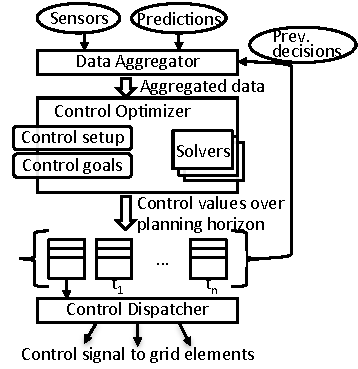
\includegraphics[width=60mm]{figures/control_flow.pdf}
  \caption{Data Flow of Hybrid Grid Control Optimization.}
  \label{fig:control}
\end{figure}
Fig. \ref{fig:control} shows the conceptual data flow. 
The flow starts with the data  aggregator. It collects data
over various data sources such as sensors, market prices, and demand 
prediction data. 
The aggregator provides a coherent view over the  grids.  
The data are then fed into the control optimizer. The optimizer
processes the data to derive best control decisions. 
The optimizer has two pre-set inputs. One input is pre-defined models
of the hybrid-grid elements and the grid structure (control setup),
and the other is the target for optimization (control target). 
The two inputs formulate constraints and objectives for mathematical
optimization, and present the control problem as an optimization
problem. 
To resolve this optimization problem, the control module employs
multiple solvers (mathematical optimizers) to search and optimize.
This includes various mathematical  programming methods (linear
programming, quadratic programming) as well as heuristic optimization
methods (such as genetic algorithm). 
Once the solvers resolve the problem, the optimizer outputs the
best control values for the planning horizon. 
%This represents the best control planning of the module at current
%moment on the grid elements. 
The next step is dispatching of the control values. The dispatcher
sends currently needed control values to actuators, and stores
planned values to ease and reduce future problem spaces. The
optimization process is repeated, as data from sensors and prediction
are updated. For the investigation, the control is initially
implemented to repeat planning for each 15 minutes. The planning
horizon is currently fixed to 24 hours. 

Control strategy modeling is similar to modeling of actors in 
economic model, in the sense that it frames the problem with
an optimization framework. However, components in the control model
are generally more detailed and complex (e.g. non-linear) since the 
control deals with actual devices. Control's optimization behavior is 
thus heavily affected by technical constraints of grid
elements, and the control's problem space is limited to short-term
horizons. % for only within the planning horizon.  

On the contrast, economic model focuses on long-term effects such as
20 year view on the impact of a new device. 
Economic model can see and optimize far further in time by simplifying
and not modeling technical constraints that can be successfully
handled by control strategy. Thus, economic model requires technical
investigation results from control-strategy evaluation to clarify what
can be safely projected within its model as technologically sound.  

\section{Economic Modeling}
\label{sec:economy_model}
\todo{Daniel: revise as needed} 
Before novel cooperative control strategies can be implemented in real 
life, their economic feasibility has to be validated for each of the
involved stakeholders. This means that the long-term monetary benefits
for the actors participating in new control strategies need to be
verified. Thus, it is important to first get a basic
understanding of the general structure of hybrid energy retail
markets.

\subsection{Market Structure}
\label{sec:econ-1}
\noindent
The most important market participants in energy retail markets are
customers (pro-/consumers), supply companies, and DSOs. Their
major interactions, roles and typical objectives are illustrated in
Fig  \ref{fig:market_structure}. 
Starting from the right-hand side, the customers try to minimize their
cost for meeting their demand for energy services, like e.g. lighting,
heating, cooling etc. Depending on their available technology
portfolio they can satisfy parts of their demand with self-generation,
and the remaining residual load has to be purchased from a supply
company via distribution networks. 
% GN: Anett recommended to change "residual load" => "residual
% demand". But this also need to change the figure, too. 
% eh, too late for now. Maybe on final manuscript. 
Supply companies retail energy in form of electricity, gas or heat to
their customers and try to maximize their profit. They can procure
this energy either by operating generation plants, by buying energy
from wholesale markets or with long-term contracts (e.g. long-term gas
delivery contracts). Of course they can also increase their profit by
selling energy on wholesale markets. 
DSOs are providing the necessary infrastructure for energy
delivery. They are responsible for (re-)investments in their
distribution networks and for the maintenance of the network
components. Network operation is characterized by economies of scale,
subadditivity of cost and sunk cost, which makes it a natural
monopoly \cite{auer_2011}. Thus, DSOs have to be regulated by a public
authority in order to ensure economic efficiency, security of supply
and non-discriminatory third-party access to the grids.  

\begin{figure}[t]
  \centering
  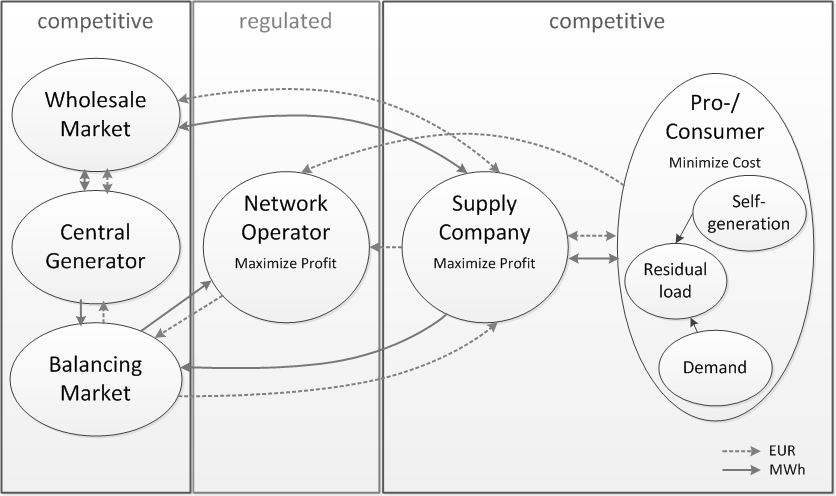
\includegraphics[width=75mm]{figures/market_structure.png}
  \caption{Simplified Illustration of the Structure of Energy Retail
    Market.}
  \label{fig:market_structure}
\end{figure}

\subsection{Methodology}
\label{sec:econ-2}
\noindent
In most cases, novel cooperative control strategies require clearly
defined business models. Here it has to be specified which market
participants are involved and how their role and responsibilities in
these new business models are allocated. It has to be described which
technology portfolio is considered in the business model and which
technologies are controlled by the control strategy in which
way. Furthermore, it is important to clearly define the ownership of
the technology portfolio
% - in some cases leasing models may be
%considered - 
and to decide who operates the controller. 
In addition,
if the controller reacts on price signals, the tariff design has to be
specified.
% Considered tariff types comprise flat tariffs, time-of-use
%tariffs (TOU), real-time-pricing (RTP), two-part tariffs and
%peak-load-pricing. 

Once the control strategy and the corresponding business model are
clearly defined, an economic trade-off analysis 
%in comparison with the
%status quo 
has to be conducted. In order to fulfill the cooperative
concept, a  crucial condition here is a Pareto-criterion. This
requires that no market participant has higher cost (or lower profit)
% –
%depending on the respective objective – 
with the new business model
than with the status quo. Thus, the formal framework for economic
modeling consists of individual optimization problems for all
involved market participants. 

\subsection{Economic Models}
\label{sec:econ-3}
\noindent
Since different hybrid control strategies and business models for
different market participants are analyzed, the economic models have
to be capable of considering various technology portfolios, several
tariff designs and multiple energy domains. To incorporate the hybrid
point-of-view, all quantities $\mathbf{q}=(q^E, q^G, q^H )^T$ and prices $\mathbf{p}=(p^E, p^G, p^H )^T$ are written as
three-dimensional vectors,
%\begin{equation*}
%  \mathbf{q}=(q^E, q^G, q^H )^T , \mathbf{p}=(p^E, p^G, p^H )^T , 
%\end{equation*}
with each component representing one energy domain: electricity,
gas and heat. Depending on the research question, control strategy and
business model, the optimization problems have different time periods,
time resolutions and are either formulated as Linear Programmings
(LPs) or Mixed Integer Linear Programmings (MILPs), if investment
decisions are considered. In the following, the considered
time period in years is written as $N$, the number of time steps per
year is denoted by $n$ and $r$ is the personal interest rate of each
market participant. 


\subsubsection{Customers}
\noindent
To minimize their cost for meeting their energy demand, customers
generally have several possibilities. They can either procure all the
energy from a supply company via the energy distribution networks at a
certain tariff or they can invest in different technologies for energy
self-generation, conversion and storing.
% In addition they can also
%invest in energy efficiency measures, like e.g. wall insulation, to
%reduce their demand. 
If the demand of a standard passive customer is
denoted by $\mathbf{d}$, and the tariff by $\mathbf{p}$, then the cost is given by 
\begin{equation}
  C = \sum_{y=1}^{N}(1+r)^{-y} \cdot \sum_{t=1}^{n} \mathbf{p}(y,t)^{T} \cdot \mathbf{d}(y,t)
\end{equation}

If a prosumer is considered, this cost function can be gradually
extended to an optimization model by adding new terms and constraints,
describing additional technologies. Consider, e.g., a customer with a
heat pump and let the energy input vector of the heat pump be denoted
by $\mathbf{q}_{in}^{HP}$, the output by $\mathbf{q}_{out}^{HP}$ and the matrix,
describing the coefficient of performance, $\mathbf{COP}^{HP}$. Furthermore,
$\mathbf{q}$ describes the energy purchased from a supply company and the
investment cost of the heat pump are given by $I^{HP}$. Then the
optimization problem of this customer can be written as: 
%\begin{align*}
%  & \min & \sum_{y=1}^{N}(1+r)^{-y} \cdot \sum_{t=1}^{n} \mathbf{p}(y,t)^T &\cdot
%  \mathbf{q}(y,t) - I^{HP}, \\
%  & \textrm{s.t.}  & \mathbf{q}(y,t) + \mathbf{q}_{out}^{HP} (y,t)&  = \mathbf{d}(y,t) +
%                     \mathbf{q}_{in}^{HP} (y,t), \\
%  & & \mathbf{q}_{out}^{HP}(y,t) & = \mathbf{COP}^{HP} \cdot \mathbf{q}_{in}^{HP} (y,t), \\
%  & & \mathbf{q}(y,t), \mathbf{q}_{out}^{HP}(y,t), \mathbf{q}_{in}^{HP}(y,t) & \geq 0.
%\end{align*} % TODO? make a better align?
\begin{align}
  & \min \sum_{y=1}^{N}(1+r)^{-y} \cdot \sum_{t=1}^{n} \mathbf{p}(y,t)^T \cdot
  \mathbf{q}(y,t) - I^{HP}, \\
  & \textrm{s.t. } \mathbf{q}(y,t) + \mathbf{q}_{out}^{HP} (y,t)  = \mathbf{d}(y,t) +
                     \mathbf{q}_{in}^{HP} (y,t), \\
  & \phantom{\textrm{s.t. }}\mathbf{q}_{out}^{HP}(y,t) = \mathbf{COP}^{HP} \cdot \mathbf{q}_{in}^{HP} (y,t), \\
  & \phantom{\textrm{s.t. }}\mathbf{q}(y,t), \mathbf{q}_{out}^{HP}(y,t), \mathbf{q}_{in}^{HP}(y,t) \geq 0.
\end{align} % TODO? make a better align? Does this look better?
In a similar way other energy conversion technologies as well as
energy generation and storage systems can be added to the model. 

The customer tariff consists of three parts, namely, (i) the energy
tariff, which is paid to the supply company, (ii) network charges,
which are paid to the distribution system operator, and (iii) fees and
taxes. Each of these parts, in general, can have several components:
(i) a one-time initial payment or connection cost, (ii) an annual lump
sum, (iii) a quantitative component, which can be flat, time-of-use (TOU) or real-time-pricing (RTP),
and (iv) a peak-load-pricing component; in order to incorporate these
different tariff types in the models, various objective terms and
constraints have to be added, which will not be further elaborated
here. 

\subsubsection{Supply Companies}
\noindent
The supply company model has a very similar structure to the customer
model. The objective is given by the firm’s profit. The revenue is
determined by the quantities, retailed to the customers at a certain tariff
%, multiplied by
%the tariff, set in the business model design, 
and possible sales on
wholesale markets.
% multiplied by the respective market prices.
The
total cost consists of the investment cost and operational cost for
generation plants, coupling technologies and energy storage
devices. Additionally, if the supply company is buying energy from
wholesale markets or via long-term contracts, these expenses have to
be considered. If the purchased energy is transmitted via a network
and if it is used by a device at the supply company’s site, e.g. a gas-fired CHP
%fired by gas
, network charges have to be paid as well. Otherwise, the
network charges are applied to the customers, consuming the energy. 

Furthermore, supply companies have to predict their generation and
their customers’ demand and report the respective schedules to a
clearing and settlement agency. If balancing energy is required to
uphold smooth network operation, they have to pay a share of the
resulting cost ex post, based on their deviations from the announced
schedule. 

Though the models for customers and supply companies presented here
are strictly cost-optimizing, they are adapted to match the operation
mode of the respective control strategy for business model
evaluation. 

\subsubsection{Distribution System Operators}
\noindent
It has already been mentioned that DSOs are regulated. Within the
regulatory constraints, however, they try to maximize their
profit. Their revenue is given by the network charges of their
customers, also including supply companies, and their cost consist of
investment cost and operational (maintenance) cost for the network
components. The DSO model is formulated as a mixed-integer
investment-planning problem, where the annual decision options
comprise reinvesting, repairing or doing nothing per component. The
realized choices affect the expected failure rate, the cost and the
total asset value, which could be subject to regulatory constraints. 

Different regulatory frameworks provide incentives for different
investment and maintenance strategies. Price- or revenue-cap
regulations limit the annual revenue and typically facilitate
under-investments. Cost-of-service or rate-of-return regulations limit
the profit by a percentage of the investments and, thus, rather
promote over-investments \cite{auer_2011}.

\section{Holistic Investigation Process}
\label{sec:holistic_investigation}
\todo{Gil: revise accordingly; reduce and mention prev. 
  sections. replace figure.}  

The investigation process as whole can be now explored, with the two
introduced components of economic and control models.

\begin{figure}[t]
  \centering
  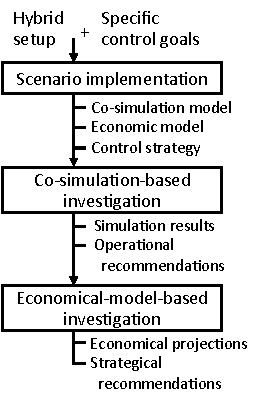
\includegraphics[width=40mm]{figures/holistic_flow.pdf}
  \caption{The flows of Holistic Investigation (figure to be replaced)}
  \label{fig:flow}
\end{figure}

%% (with new figure) add description on the figure. 

\paragraph{Defining scenario.} 
\noindent
The investigation starts by designing a specific hybrid evolution
scenario. In this paper, a {\em scenario} means a hybrid setup of Table
\ref{tab:1} instantiated into a concrete situation, bounded by
specific control goals and hybrid devices. For example, {\em 
  Co-operative suppliers} setup of Skellefte{\aa} can be turned into a 
scenario of ``providing better peak-boiler with hybrid strategy'', by
adding electric boilers in addition to existing CHP and oil peak
boilers. The control goal for the scenario can be: a) best cost
peak-heat supply by tapping into fluctuating electricity price, and b)
reduce total green-house gases. Finally, attaining the goals would
require new control strategies.  
This would form a concrete investigation scenario that can be clearly
evaluated and compared with current state-of-the-art.  

\paragraph{Scenario implementation.} 
\noindent
Once a scenario is given, the next step is {\em Scenario
  Implementation}. This includes building the simulation models 
for the target site, implementing the control model that meets the
control goal, and the instantiation of the economic model that can
describe the major actors of the scenario. 
If we follow the example of  ``better peak-boiler'' scenario,
simulation models to be implemented are district heat grid simulation
and electricity grid simulation of the target site, where the two
simulations are to be run by a co-simulation tool. A control model is
implemented to control the simulated components on the simulation;
such as CHP, added electric boilers, oil boilers, heat storage, power
grid switches and so on. The economic model incorporates major
contributors of the scenario, including major devices (above mentioned
CHP and boiler behaviors, simplified), and stakeholders' behavior (the
expected long-term behavior of power and heat providers). 

\paragraph{Simulation-based investigation.} 
\noindent
The next step is {\em Co-simulation-based investigation}. 
This step is characterized by many simulation runs for testing the
control strategies. 
Each competing control strategy (including baseline) is being
evaluated over the target grids in various relevant situations. 
Continuing the example of peak-boiler scenario, a set
of control strategies will be evaluated across various demand
conditions (e.g. cold, not-so-cold winter), price conditions (high/low
price ratio of oil to electricity), various boiler sizes (adding
single to multiple electricity to heat devices), for many simulated
winter months. The investigation step systemically covers as many 
combinations as possible to make fair comparisons.   

Note that it is a co-simulation environment. In a co-simulation, each
simulation (e.g. heat grid and power grid simulation) runs together
and exchange information at the same time, bounded by a co-simulation
tool. 
For our investigation,
PowerFactory\footnote{\url{http://www.digsilent.de/}} was used as
power grid simulation, Dymola\footnote{\url{http://www.3ds.com/products-services/catia/products/dymola
 }} for district heat simulation, and  FMI++\footnote{\url{http://sourceforge.net/projects/fmipp/}} as the 
co-simulation driver.  
Detailed description of the co-simulation environment is outside of
the scope of this paper. Interested readers are kindly asked to refer
to \cite{Widl_2015} for the environment we have adopted. 

Direct result of the simulation investigation is all values that 
are observed and saved from a simulation run. The observed values can
be processed further by technical evaluation measures, and can be
compared between different strategies and/or hybrid configurations. 
This enables investigators to form concrete conclusions with
supporting numbers and measures. In this paper, this conclusion out of
simulation investigation is called {\em Operational recommendation}. 
It includes the modeled control strategy itself (the best control
strategy among tested), and evaluated performance differences and
lessons learned from the simulation runs. 

\paragraph{Economic-model-based investigation.}
\noindent
The last step of the investigation is {\em Economic-model-based 
  investigation}. 
The simulation-based model alone cannot answer all important
questions. Long-term effects and indicators like the internal
rate-of-return (IRR) of investments need to be evaluated by an
additional economic model.   
This also includes competing interests of stakeholders. 
The economic investigation comprises an analysis of currently existing
structural barriers and the design of novel business models that
enable a distribution of benefits, where all stakeholders can profit.  

The economic model uses simulation results of the previous step
to calibrate various parameters within the model. 
By doing this calibration, it can describe realistic long term effect
of a hybrid grid strategy (such as total energy saved by a specific
control scheme, or the behavior of a specific hybrid elements in
different conditions) without explicitly modeling all technological
details of the simulation. 
On the other hand, the economic model explicitly models and provides
all major economic values and their stakeholders' interest, which are  
absent in the simulation. The values observable in economic model are
processed further by social and economic evaluation measures, which
can compare the proposed scenario with baselines. 
This enables the investigators to draw concrete conclusions for each 
proposed hybrid scenario. This conclusion, supported by projected
values and measures of economic model, is called {\em Strategic
Recommendation}. 
This provides the best perceived way of investments for the given
scenario, and their expected return, and possible (or needed)
price-scheme and business models.    


\section{Case Study on Skelleftea: Providing Better Peak  Heating via Hybridization}
\subsection{Introduction to the Hybridization Scenario} 
\todo{Gil: to write} 

\subsection{Operational Recommendations: Co-simulation based investigation results}
\todo{Gil: to write} 

\subsection{Strategic Recommendations: Economy model based
  investigation results} 
\todo{Daniel: to write}

\section{Conclusion}
\todo{Gil: Expand and Revise}
The paper proposed two-step investigation process that enables
concrete and thorough checking of hybrid energy grid scenarios. The
competitive edge of the proposed process comes from the approach's
ability to check and  sample details on both operational
(short-term, technical) and strategic (long-term, economic and
social) aspects of the given setup. It provides a set of holistic
recommendations for stakeholders of the investigated grids. It is our 
belief that the holistic recommendations will provide valuable
insights for the possible future energy grid evolution.

\section*{Acknowledgment}
We gratefully acknowledge funding and support by the European
Commission (project OrPHEuS (FP7 ICT-608930)). 

%\section*{References}

%\bibliography{mybibfile}
\bibliography{orpheus_AE.bib}

\end{document}